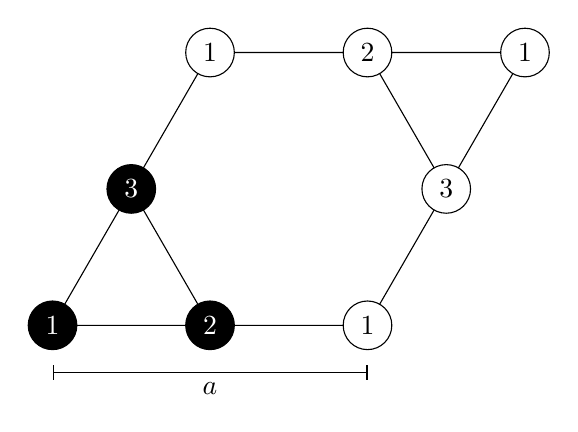
\begin{tikzpicture}[
        atom/.style={fill=black, circle, text=white, draw},
        ghost/.style={fill=white, draw, circle},
        scale=2,
    ]
    \draw (60:1) -- ++(-60:1);
    \draw (60:1) ++(0:2) -- ++(120:1);

    \draw (0, 0) node[atom] {1}
    -- ++(60:1) node[atom] {3}
    -- ++(60:1) node[ghost] {1}
    -- ++(0:1) node[ghost] {2}
    -- ++(0:1) node[ghost] {1}
    -- ++(60:-1) node[ghost] {3}
    -- ++(60:-1) node[ghost] {1}
    -- ++(0:-1) node[atom] {2}
    -- ++(0:-1);

    \draw[|-|] (0, -.3) -- ++(2, 0) node[midway, below] {$a$};
    
\end{tikzpicture}
